\section{Resumen ejecutivo y alcance documental}
El repositorio \code{AiGB_UEx_Navigation_v2} integra simulación física, adquisición sensorial, estimación probabilística de pose, percepción semántica y navegación de una plataforma Husky en un huerto de manzanos. Su resultado perceptivo es un mapa semántico incremental: los objetos observados se representan como plantas o personas, las plantas alineadas se agrupan en filas y las filas compatibles se organizan en parcelas. Estas entidades se publican en una memoria de trabajo distribuida que también contiene transformaciones espaciales y propuestas de acción.

La revisión de esta versión se fundamenta en archivos de implementación y configuración, identificados en la sección de trazabilidad. El README general conserva descripciones anteriores a la unificación de tronco y dosel en \code{plant_concept}; por ello se concede prioridad al código y a \code{conceptos.md} para describir el estado actual. La inspección activa está implementada. La conservación de un mapa de referencia entre sesiones y la relocalización sobre dicho mapa constituyen desarrollos pendientes en la documentación revisada. No se confunden estas capacidades con la creación de nodos durante una ejecución.

El presente documento es un borrador técnico de desarrollo. La existencia de código se diferencia de su validación experimental: no se presentan prestaciones de campo, tasas de éxito ni precisiones obtenidas en campañas que no se hayan documentado con registros reproducibles.

\section{Fundamentos de la arquitectura}
\subsection{RoboComp y organización en componentes}
RoboComp proporciona la infraestructura para construir programas robóticos distribuidos que intercambian datos mediante interfaces definidas. En el proyecto, cada componente dispone de configuración, ciclo de ejecución y servicios propios. Esta separación permite ejecutar el simulador, los drivers, la percepción y el controlador como procesos diferentes. Los archivos de configuración determinan conexiones y parámetros; los lanzadores coordinan su inicio.

Un componente no equivale necesariamente a un sensor físico. Por ejemplo, el puente Webots expone sensores simulados, mientras que \code{plant_concept} integra evidencia procedente de varios sensores para mantener una entidad del entorno. El ciclo de una aplicación depende tanto de la disponibilidad de sus entradas como de las condiciones del grafo.

\subsection{CORTEX y DSR}
CORTEX es una arquitectura cognitiva basada en agentes que comparten una representación dinámica del entorno. La estructura que desempeña el papel de memoria de trabajo se denomina \emph{Deep State Representation} (DSR). La denominación utilizada por la biblioteca es DSR; ``DER'' no corresponde al nombre del mecanismo empleado. CORTEX designa la organización arquitectónica y DSR la representación que utilizan sus agentes \cite{cortex}.

Formalmente, se considera un grafo dirigido y atribuido
\begin{equation}
G=(V,E,A_V,A_E),
\end{equation}
donde los nodos $V$ representan entidades, las aristas $E$ expresan relaciones y los atributos $A_V,A_E$ contienen propiedades numéricas, simbólicas o geométricas. Una planta dispone de identidad, partes observadas y posición; una fila dispone de orientación, extensión y miembros. El grafo es híbrido porque reúne geometría y significado en una misma estructura.

Cada agente mantiene una réplica local. La infraestructura CORTEX propaga cambios de estado mediante tipos de datos replicados libres de conflictos (CRDT). La consistencia eventual implica que las réplicas convergen cuando cesan las modificaciones y se propagan sus cambios; no implica que todos los agentes lean un estado global idéntico en cada instante. Esta distinción motiva comprobar timestamps, existencia de nodos y validez de transformaciones antes de utilizar datos \cite{cortex}.

La propiedad de entidades complementa la consistencia del transporte. \code{plant_concept} escribe las plantas y \code{row_metaconcept} las filas. Los demás agentes consumen esas representaciones. Los CRDT resuelven la convergencia de datos, pero no deciden si dos estimaciones físicas contradictorias son correctas.

\subsection{DDS, Ice y dos niveles de intercambio}
DDS significa \emph{Data Distribution Service}. Se utiliza como comunicación de publicación y suscripción: un productor publica muestras de un tipo en un tópico y los lectores compatibles reciben esas muestras. Los dominios separan espacios de comunicación, mientras que las políticas de calidad de servicio regulan aspectos como fiabilidad e historial. El proyecto utiliza tecnología eProsima tanto en infraestructura distribuida como en canales sensoriales; su configuración concreta depende de cada componente \cite{cortex,launch}.

Ice proporciona interfaces de objetos remotos: un componente invoca una operación de otro mediante un proxy y un endpoint. La configuración del Husky expone la base y GPS mediante el puente y utiliza drivers para trasladar sensores al plano DDS. El joystick emplea también publicación mediante IceStorm. No todos los mensajes atraviesan una misma interfaz.

Deben distinguirse dos intercambios: las imágenes, nubes y muestras inerciales alimentan el procesamiento sensorial; los nodos, relaciones y atributos DSR comunican el conocimiento producido. Publicar una imagen por DDS no crea por sí solo una planta. La transformación de medida a concepto se realiza mediante los algoritmos de percepción.

\section{Plataforma física simulada y escenarios}
El modelo \code{HuskyA300.proto} representa una base de cuatro ruedas skid-steer. Su marco corporal utiliza $+Y$ hacia delante, $+X$ hacia la derecha y $+Z$ hacia arriba. Los sensores incluyen LiDAR Helios, cámara ZED, IMU y GPS. Sus extrínsecos relacionan cada dispositivo con la base. Estos desplazamientos deben conservarse: la posición GPS corresponde a la antena y no directamente al origen del robot.

\code{AppleTree.proto} genera un manzano de eje central con tronco, ramas, hojas, frutos y tutor opcional. La semilla determina la geometría de cada ejemplar. Se emplean mallas agrupadas para reducir el número de objetos gráficos. La geometría visible y la de colisión cumplen funciones diferentes: el modelo original limita la colisión física al tronco, mientras que hojas, frutos y ramas contribuyen a la imagen y a la geometría observada por el sensor simulado. Esto limita la interpretación de contactos con vegetación \cite{sim}.

\code{gen_apple_rows.py} distribuye individuos con perfiles de tamaño y vigor y permite reproducir hileras. Los mundos \code{husky_apple.wbt} y \code{dos_fields.wbt} proporcionan escenarios distintos. La cantidad exacta de árboles y sus coordenadas se obtiene del archivo de mundo usado en cada ensayo; no se presupone que los comentarios históricos del README describan todas sus revisiones.

\begin{figure}[htbp]
\centering
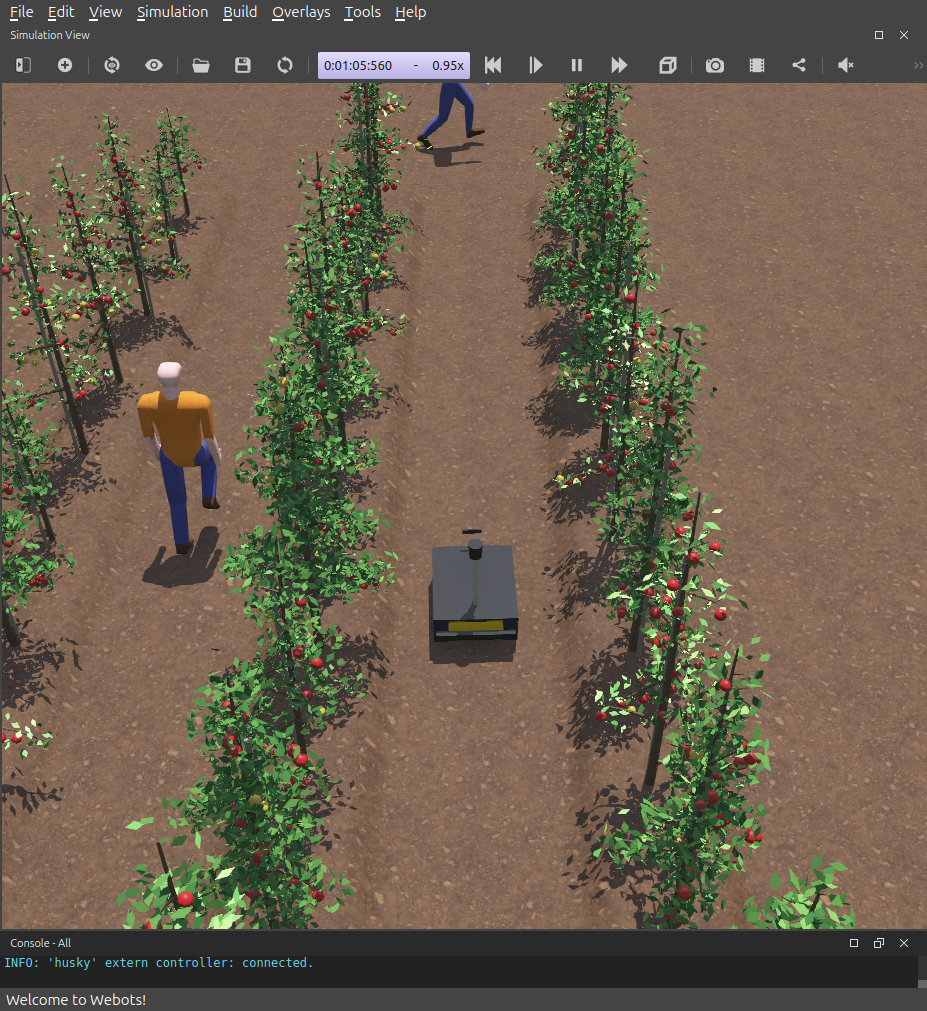
\includegraphics[width=0.82\linewidth]{../images/01_webots_simulator_navigating.png}
\caption{Captura preexistente del repositorio: Husky en el huerto simulado. Se utiliza como ilustración de la plataforma; no constituye un resultado de una campaña nueva.}
\end{figure}

\section{Cadena de adquisición y procesamiento}
\subsection{Inicio y dependencias}
El lanzador de escenario inicia Webots, la capa sensorimotora y la capa cognitiva. \code{sub_husky.toml} declara el puente, LiDAR, IMU, cámara y joystick. \code{cognitive_husky.toml} declara los agentes perceptivos y de navegación. El orden de lanzamiento prepara las dependencias, pero la disponibilidad efectiva depende de los estados de operación y de las entradas de cada agente \cite{launch}.

\code{robot_concept} introduce la descripción del cuerpo y sensores. \code{openfield_concept} espera las medidas necesarias para inicializar su estimador y establecer el campo. Los agentes perceptivos necesitan resolver las transformaciones entre sensores, robot y campo antes de publicar posiciones coherentes. El controlador utiliza los obstáculos y límites disponibles para producir órdenes de movimiento.

\subsection{Puente y sensores}
El puente accede a dispositivos de Webots y expone sus medidas mediante interfaces RoboComp. El driver LiDAR procesa la nube y publica el flujo correspondiente; el driver IMU traduce las muestras inerciales al plano de datos; la cámara proporciona imágenes y geometría asociada para percepción. La configuración sensorimotora documenta el dominio 7 y el tópico \code{rc/imu/data} para la IMU. Las direcciones, tópicos y frecuencias restantes se deben obtener de sus TOML específicos, pues no son propiedades universales de DDS.

El instante de adquisición y el marco de referencia forman parte del significado de una medida. Una nube capturada mientras el robot gira no puede proyectarse sin considerar la pose correspondiente. La presencia de timestamps facilita el alineamiento, aunque no demuestra por sí sola sincronización perfecta entre todos los canales.

\subsection{Percepción visual}
\code{retina} procesa las imágenes con modelos configurados para segmentación semántica, segmentación de personas y pose humana. Las máscaras seleccionan píxeles compatibles con clases de interés. La profundidad y la calibración permiten convertirlos en puntos tridimensionales. En un modelo pinhole, la desproyección se expresa como
\begin{equation}
\mathbf p_C=zK^{-1}[u,v,1]^\mathsf T,
\end{equation}
donde $K$ representa los intrínsecos, $(u,v)$ el píxel y $z$ su profundidad axial. Esta expresión describe la operación geométrica; las convenciones y conversiones efectivas deben coincidir con el driver.

La segmentación de vegetación constituye evidencia para el agente de plantas. La segmentación y los esqueletos humanos alimentan a \code{human_concept}. Una etiqueta semántica aislada no implica existencia confirmada ni posición estable de una entidad.

\section{Marcos espaciales y localización del Husky}
\subsection{El campo como lugar y referencia}
En la revisión actual desaparece el nodo exterior \code{world}. El nodo \code{field}, propiedad de \code{openfield_concept}, representa simultáneamente el lugar de trabajo y su marco de coordenadas. Contiene el polígono operativo, el estado de inspección y relaciones con parcelas. El marco horizontal emplea este y norte en la configuración geográfica exterior. El antiguo \code{field_metaconcept}, que producía un campo separado, queda obsoleto según el contrato revisado \cite{conceptos}.

La transformación publicada se almacena en la arista \code{robot -> field}. Si $T_{F\leftarrow R}$ expresa la pose del robot en el campo, la arista almacena su inversa $T_{R\leftarrow F}$. Para un punto sensorial:
\begin{equation}
\mathbf p_F=T_{F\leftarrow R}T_{R\leftarrow S}\mathbf p_S.
\end{equation}
La dirección del enlace del grafo y la interpretación de la pose deben distinguirse para evitar inversiones duplicadas.

Los nodos de planta, fila y parcela se posicionan directamente respecto a \code{field}. La pertenencia semántica se expresa mediante \code{group_member}; no mediante una cadena espacial parcela--fila--planta. Por tanto, cambiar la pertenencia de una planta no obliga a desplazarla físicamente.

\subsection{Filtro extendido de Kalman}
El estimador utiliza el estado $\mathbf x=[x,y,\theta]^\mathsf T$ y su covarianza $P$. La predicción combina velocidades de ruedas y velocidad angular del giróscopo. Con $v_a$ hacia delante, $v_s$ lateral y $\bar\theta=\theta+\omega\Delta t/2$, la implementación integra \cite{ekf}:
\begin{align}
x^+&=x+(v_s\cos\bar\theta-v_a\sin\bar\theta)\Delta t,\\
y^+&=y+(v_s\sin\bar\theta+v_a\cos\bar\theta)\Delta t,\\
\theta^+&=\operatorname{wrap}(\theta+\omega\Delta t).
\end{align}
El uso del giróscopo para el giro evita depender exclusivamente del giro inferido de ruedas en una base que puede deslizar. El ruido de proceso depende de velocidad y maniobra; su efecto se propaga con los jacobianos del modelo.

La medida GPS se compara con la posición predicha de la antena:
\begin{equation}
h_{GPS}(\mathbf x)=\begin{bmatrix}x\\y\end{bmatrix}+R(\theta)\boldsymbol\ell,
\end{equation}
donde $\boldsymbol\ell$ es el brazo de palanca. El yaw absoluto de la IMU proporciona otra corrección. La actualización EKF utiliza innovación, covarianza de innovación y ganancia de Kalman; por ello tanto la precisión sensorial como la incertidumbre previa afectan al resultado.

La configuración examinada usa \code{GpsSigmaSource="fixed"}, \code{GpsLikelihood="gauss"}, desviación GPS de 0.05 m y compensación temporal desactivada. Existen alternativas de incertidumbre del receptor y verosimilitud Student-t para reducir la influencia de saltos, pero su disponibilidad no significa que estén activas. La incertidumbre configurada es un supuesto del filtro, no una precisión demostrada en campo.

\section{Creación incremental del mapa semántico}
\subsection{Definición operacional}
El mapa semántico se crea cuando las observaciones se convierten en entidades identificables con geometría y relaciones. La secuencia implementada es: adquisición, segmentación, desproyección, transformación al campo, acumulación de evidencia, asociación temporal, creación o actualización de plantas e inferencia de filas y parcelas. El grafo resultante permite responder qué existe, dónde está y cómo se organiza.

Esta construcción utiliza la pose estimada para ubicar las entidades. No demuestra que esas entidades estén corrigiendo la pose. La interfaz del EKF revisado utiliza GPS, yaw y movimiento; la localización contra un mapa persistente de filas pertenece a la extensión descrita en \code{mapeo.md}.

\subsection{Hipótesis y confirmación del tronco}
El submodelo \code{trunk_map} de \code{plant_concept} recibe evidencia visual de vegetación en una banda baja, documentada alrededor de 0.30--0.55 m. Los candidatos se agrupan espacialmente y se contrastan con retornos LiDAR en la banda compatible. Esta combinación reduce la dependencia de una máscara visual aislada. Los parámetros de agrupación, confirmación y ruido pertenecen a la configuración del modelo \cite{plants}.

La existencia se mantiene mediante evidencia acumulada y pruebas de visibilidad. Una ausencia aporta información solo cuando el sensor debería haber observado el tronco; una oclusión por hojas o personas no equivale a desaparición. El modelo emplea contribuciones de evidencia positiva y negativa, moduladas por visibilidad.

El radio físico se estima mediante la dispersión lateral de puntos LiDAR sobre la silueta. Bajo la hipótesis utilizada por el modelo, el radio se aproxima por dos veces la mediana del valor absoluto de los desplazamientos laterales. El procedimiento incluye separación del tutor cuando existe un hueco observable y acumulación entre barridos. Esta estimación depende de resolución, distancia, oclusión y geometría; no constituye una garantía universal de exactitud.

\subsection{Acumulación de evidencia del dosel}
El submodelo \code{vegetation_map} proyecta puntos de máscaras vegetales sobre una rejilla horizontal dispersa. Se descartan alturas incompatibles con vegetación para reducir contaminación del suelo o cielo. Cada celda recibe evidencia por las observaciones que la alcanzan; múltiples píxeles del mismo fotograma no se cuentan como observaciones independientes. La ponderación temporal limita además el efecto de incrementar la frecuencia de procesamiento \cite{plants}.

Los centros de dosel se obtienen mediante \emph{mean shift} con un núcleo de disco sobre la evidencia acumulada. Una concentración suficiente permite crear una hipótesis. El modelo emplea discos de radio configurado; por tanto, el radio del dosel publicado no debe interpretarse automáticamente como un ajuste libre de toda su superficie. Las hipótesis solapadas se consolidan preservando identidad anterior. La evidencia de dosel se acumula sin un mecanismo simétrico de retirada en el modelo revisado.

Una observación desde un único pasillo puede desplazar el centro aparente hacia la cara visible de la copa. Nuevas vistas pueden modificarlo. Esta diferencia es relevante para asociar observaciones aéreas y terrestres: centro del dosel y eje del tronco no son necesariamente coincidentes.

\subsection{Composición de una planta individual}
\code{PlantComposer} asocia troncos y doseles. Se consideran parejas en las que el tronco queda dentro del disco del dosel; se ordenan por distancia y se seleccionan correspondencias uno a uno. La planta puede existir con solo una parte. Cuando aparece la parte faltante, se incorpora al individuo existente cuando la asociación lo permite; si dos hipótesis previas se consolidan, se gestiona su absorción.

El origen de la planta corresponde al tronco cuando está disponible y, en caso contrario, al centro del dosel. Se publican atributos como \code{plant_has_trunk}, \code{plant_has_canopy}, radio del tronco, radio y desplazamiento del dosel, altura y probabilidad de existencia. La arista RT transporta la geometría y covarianza publicada. El número de nodos representa individuos, no partes: no se crea un nodo DSR por hoja o por fruto \cite{conceptos,plants}.

\subsection{Inferencia de filas}
La fila se deduce de las posiciones de plantas con tronco observado. El algoritmo de \code{rows.h} realiza las siguientes operaciones \cite{groups}:
\begin{enumerate}
\item Se identifican vecinos próximos. Se supone que la separación dentro de una fila es menor que entre filas.
\item Se estima una dirección predominante a partir de las direcciones de los vecinos. La media de ángulo doble trata una recta y su orientación opuesta como equivalentes:
\begin{equation}
\alpha=\tfrac12\operatorname{atan2}\left(\sum_i\sin 2\alpha_i,\sum_i\cos 2\alpha_i\right).
\end{equation}
\item Las plantas se proyectan sobre la perpendicular a esa dirección. Los huecos laterales separan grupos candidatos.
\item Cada grupo se ordena longitudinalmente; huecos suficientemente grandes dividen segmentos. Se requiere un mínimo configurado de miembros.
\item Se calcula el eje principal de cada segmento y un rectángulo con longitud, anchura y márgenes. La identidad se conserva mediante miembros compartidos con las filas anteriores.
\end{enumerate}
Las plantas con solo dosel pueden incorporarse como miembros cuando su posición queda dentro del rectángulo de una fila, sin reemplazar necesariamente las observaciones precisas utilizadas para inferir su eje.

Este procedimiento favorece plantaciones regulares. Filas curvas, separaciones atípicas o numerosos individuos ausentes pueden vulnerar sus hipótesis. El rectángulo incorpora márgenes de navegación: su extremo no equivale necesariamente a un extremo físico verificado del cultivo.

\subsection{Parcelas y actualización del campo}
\code{plot_metaconcept} agrupa filas aproximadamente paralelas, próximas lateralmente y con solapamiento longitudinal. La separación característica se estima con distancias a filas vecinas; una separación mayor puede originar otra parcela. Las identidades se mantienen según miembros compartidos. \code{openfield_concept} relaciona las parcelas con \code{field}. Esta jerarquía organiza el mapa sin modificar el marco espacial individual de las entidades \cite{groups,conceptos}.

\subsection{Ejemplo de construcción}
Cuando se observa una copa sin tronco, se acumula evidencia y puede nacer \code{plant_0}. La planta queda marcada como incompleta. Una observación posterior compatible del tronco permite completar el mismo individuo. Cuando aparecen otras plantas alineadas, se crea \code{row_0} y sus relaciones de pertenencia. Nuevas plantas amplían la fila; varias filas compatibles permiten inferir una parcela. El mapa surge de estas actualizaciones sucesivas, no de copiar la lista de árboles del mundo de Webots.

\section{Inspección activa y selección de observaciones}
\subsection{Modelo de cobertura}
\code{FieldExplorer} representa el polígono de misión mediante celdas. Cada celda mantiene una variable $u_c$ asociada al contenido aún desconocido. La medida de entropía utilizada por el modelo es $H_c=u_cH_0$, donde $H_0$ se obtiene del prior binario de presencia de plantas. La probabilidad de detección disminuye con distancia y con filas interpuestas \cite{explore}:
\begin{align}
p_{det}(v,c)&=\exp[-(d(v,c)/r)^2]\prod_j\tau_j,\\
u_c^+&=u_c\exp[-\kappa p_{det}\Delta t],\\
\Delta H(v)&=\sum_cH_c\{1-\exp[-\kappa p_{det}(v,c)T]\}.
\end{align}
Aquí $r$ es la escala de alcance, $\tau_j$ la transmitancia modelada, $\kappa$ la tasa de detección y $T$ el tiempo de observación. Estas cantidades constituyen hipótesis del modelo de inspección. La reducción de esta entropía modelada no demuestra que todas las plantas reales hayan sido detectadas.

\subsection{Plantas incompletas y utilidad de una vista}
El explorador también representa preguntas sobre partes no observadas. Una planta con copa pero sin tronco genera una hipótesis sobre la existencia de la parte faltante. Las observaciones que deberían verla y no la encuentran reducen esa creencia. El parámetro \code{ConceptWeight} pondera la resolución de estas preguntas respecto a cobertura.

La selección combina beneficio informativo y coste de desplazamiento. En la formulación básica se maximiza $\Delta H(v)-\lambda d(v)$, con candidatos restringidos por límites del campo, rectángulos de filas y discos de exclusión. La integración publica ganancia marginal respecto a la situación actual. La llegada a una vista y la información obtenida son eventos diferentes.

\subsection{Protocolo de affordances y finalización}
\code{OpenFieldExploration} publica \code{afford_openfield}, que contiene posición objetivo, orientación y ganancia epistémica. El protocolo coordina los estados \code{Offered}, \code{Executing} y \code{Completed}. El controlador selecciona y ejecuta la acción. La integración contempla puntos inalcanzables, expiración de ofertas y vigilancia de falta de progreso; los fallos suprimen temporalmente candidatos próximos.

El estado global evoluciona desde \code{Waiting} a \code{Inspecting} y \code{Complete}. El campo publica \code{model_stable} y \code{model_uncertainty}. La condición de terminación responde a que ninguna vista candidata justifica su coste bajo el modelo. No equivale a una certificación agronómica de exhaustividad. El polígono es una entrada de misión, obtenida de configuración o del simulador según el modo; no se aprende como el polígono de paredes de \code{room_concept}.

\section{Seguimiento de personas y evidencia dinámica}
\code{human_concept} consulta una fuente de esqueletos y crea hipótesis de persona asociadas a trayectorias. Su ciclo utiliza los cuerpos recibidos para actualizar el ajuste y la existencia de cada individuo. El código incluye un canal adicional de presencia LiDAR; su empleo depende de la configuración. La publicación de un esqueleto visual y la existencia de una persona confirmada son niveles distintos del procesamiento \cite{humans}.

La vegetación conocida condiciona la interpretación: el agente consulta discos de plantas para evitar atribuir a personas retornos que ya se explican por vegetación. La representación compartida permite así que la percepción de un concepto afecte a otro. Sin embargo, un error en la geometría vegetal puede propagarse a la interpretación de personas; deben evaluarse falsos positivos y falsos negativos cerca de copas y troncos.

La cadena de dependencias principal se resume en la figura siguiente. Las flechas representan flujo funcional, no conexiones DDS exclusivas ni orden obligatorio de procesos.
\begin{figure}[htbp]
\centering
\fbox{\begin{minipage}{0.92\linewidth}\centering
Webots y sensores simulados\\[2mm]
$\downarrow$\\
Puente y drivers: imágenes, nubes, IMU, GNSS y movimiento\\[2mm]
$\downarrow$\\
Estimación de pose y percepción visual\\[2mm]
$\downarrow$\\
Plantas y personas $\longrightarrow$ filas $\longrightarrow$ parcelas\\[2mm]
$\downarrow$\\
Memoria DSR: entidades, transformaciones, pertenencia y affordances\\[2mm]
$\downarrow$\\
Inspección y navegación $\longrightarrow$ nuevas observaciones
\end{minipage}}
\caption{Cadena funcional de construcción y uso del mapa semántico. La memoria DSR interviene en varios pasos y no únicamente al final.}
\end{figure}

\section{Navegación y tratamiento del espacio residual}
El mapa semántico explica objetos conocidos, pero no todos los retornos sensoriales corresponden a una entidad reconocida. \code{residual_concept} representa evidencia no explicada mediante ocupación. Esta capa permite que un obstáculo desconocido influya en navegación antes de disponer de una categoría semántica.

El controlador combina límite operativo, ocupación residual y geometría de exclusión. Las filas se utilizan como rectángulos no transitables; para plantas no agrupadas se emplean discos del tronco. Los márgenes de exclusión expresan necesidades de movimiento y no dimensiones botánicas medidas.

\code{GridPlanner} implementa búsqueda A* sobre una rejilla y comprueba colisión con la huella del robot. La configuración incorpora preferencias de separación de obstáculos. El plan se utiliza en el control de trayectoria y la producción de órdenes de base. La cadena debe considerar antigüedad de datos y ausencia de rutas, ya que un objetivo válido en el grafo puede resultar inalcanzable para la geometría actual \cite{nav}.

El README registra bloqueos por obstáculos fantasma asociados a inclinación del Husky y suelo elevado. La hipótesis de pose plana y un umbral de altura respecto a un suelo global pueden interpretar un bancal como obstáculo. El diagnóstico debe verificarse con las transformaciones y registros de cada ejecución; una imagen del planificador no permite atribuir por sí sola la causa a percepción o control.

\section{Extensión aérea y estado de integración}
El repositorio contiene un mundo derivado con dron, cámara orientable y plataforma con marcador. Además, la revisión del código identifica \code{webots-drone-bridge}, que adquiere imágenes, controla actuadores y publica RGB mediante DDS. Por tanto, la descripción histórica de una incorporación exclusivamente de hardware ya no resume todo el código disponible \cite{drone}.

El puente inspeccionado obtiene posición y velocidad mediante el supervisor de Webots y calcula transformaciones entre portador, dron y cámara. Las marca con origen \code{webots-supervisor} y estado simulado. Estas transformaciones son información privilegiada del simulador; no constituyen una estimación visual/GNSS validada. Su empleo es adecuado para comprobar integración geométrica, pero los resultados deben distinguirse de los obtenidos con localización estimada.

La cámara orientable introduce una transformación variable que debe acompañar a cada captura. La existencia de un ArUco sobre la plataforma no acredita detección o aterrizaje autónomo. Para demostrar estas funciones se requiere documentar el estimador relativo, su incertidumbre, el control de descenso y la reacción ante pérdida del marcador. La mera presencia del directorio de puente tampoco demuestra su activación en todos los lanzadores.

\section{Procedimiento reproducible de ejecución y evaluación}
\subsection{Registro de condiciones}
Cada ejecución debe identificarse mediante revisión del código, mundo, configuración, semillas, modelos de percepción y versiones de dependencias. Se conserva el estado de GNSS y el modo de inspección. La denominación de un escenario no sustituye sus parámetros: dos revisiones de \code{dos_fields.wbt} pueden contener disposiciones distintas.

\subsection{Preparación y ejecución}
El procedimiento operativo comprende la compilación de los componentes declarados, disponibilidad de pesos de percepción, inicio del mundo y lanzamiento de capas. Los scripts existentes permiten iniciar escenarios y detener procesos; las opciones se consultan en la versión utilizada. Durante la adquisición se registran pose estimada, covarianza, medidas sensoriales, creación de entidades, cambios de pertenencia y transiciones de affordances. La activación de \code{Diag.ExperimentCsv} determina si se genera el registro experimental adicional del estimador.

La campaña propuesta comienza con GNSS nominal y recorrido repetible; posteriormente varía disponibilidad/calidad de GPS, apariencia vegetal y terreno. Para estudiar inspección se registra el orden de objetivos, vistas alcanzadas, fallos, ganancia estimada y contenido observado. Para el dron se registra por separado si la pose procede del supervisor o de un estimador.

\subsection{Métricas y evidencia necesaria}
\begin{longtable}{p{0.22\linewidth}p{0.68\linewidth}}
\toprule Área & Métricas propuestas \\\midrule
Localización & Error lateral, longitudinal y angular; consistencia de la covarianza; recuperación tras pérdida de GNSS. \\
Mapa semántico & Precisión y exhaustividad de plantas; duplicados; error de posición y radio; asignación correcta de miembros a filas. \\
Filas & Error angular, desplazamiento lateral, extensión y estabilidad de identidad entre pasadas. \\
Inspección & Cobertura observada, hipótesis pendientes, distancia y tiempo; diferencia entre ganancia prevista y observación real. \\
Navegación & Llegadas, objetivos inalcanzables, intervenciones, separación de obstáculos y tiempo de ciclo. \\
Integración aérea & Latencia de imagen, coherencia temporal de pose, error de transformación y observabilidad del marcador. \\
\bottomrule
\end{longtable}
La verdad de Webots se utiliza como referencia de evaluación cuando se mide autonomía perceptiva. Si un módulo consume esa verdad, el ensayo debe declararse como integración con estado conocido. Las repeticiones y condiciones adversas se reportan individualmente antes de agregar promedios. No se incluyen resultados numéricos nuevos en este documento, pues su redacción se ha realizado mediante inspección de fuentes.

\section{Limitaciones, persistencia y desarrollo previsto}
El mapa de la sesión, la cobertura modelada y el mapa persistente son productos diferentes. La configuración actual permite crear entidades y finalizar una inspección; esto no implica guardar una referencia compacta ni recuperar identidades entre reinicios. La propuesta de persistencia conserva geometría de filas, extremos verificados, incertidumbre y referencias individuales cuando sean necesarias para resolver simetrías.

La navegación basada en filas presenta una limitación de observabilidad: líneas paralelas restringen orientación y desplazamiento lateral, pero aportan poca información longitudinal. El GPS o extremos observados pueden resolver parte de la ambigüedad. Si se incorporan filas para corregir pose, deberán emplearse observaciones relativas y controlarse las correlaciones: una fila obtenida con la pose actual no puede reutilizarse como referencia independiente y exacta.

La representación de dosel mediante radio fijo, la ausencia de retirada simétrica de su evidencia y la dependencia de la geometría de plantación deben evaluarse antes de transferir el sistema al campo. Frutos, malezas y daños requieren además modelos y anotaciones específicas. La presencia de manzanas renderizadas en Webots no equivale a un canal cognitivo validado de conteo o diagnóstico.

\section{Trazabilidad de la descripción}
Las referencias siguientes identifican las fuentes locales revisadas. Las rutas son relativas a la raíz del repositorio salvo indicación contraria. Se conservan como guía para actualizar el informe cuando cambie la implementación. La bibliografía bibliográfica heredada permanece en \code{bibliografia.bib}; no se añaden citas que no respalden una afirmación utilizada.
\begin{thebibliography}{99}
\bibitem{cortex} RoboComp. \emph{CORTEX and DSR (Deep State Representation)}. README de la instalación local \path{/home/nosl3n/robocomp/cortex/README.md}. Repositorio: \url{https://github.com/robocomp/cortex}.
\bibitem{launch} Configuración de lanzamiento: \path{active_inference/utils/sub_husky.toml} y \path{active_inference/utils/cognitive_husky.toml}.
\bibitem{conceptos} Contrato de conceptos del huerto: \path{active_inference/conceptos.md}. Revisión con migración a \code{field} de 2026-11-04.
\bibitem{sim} Modelo de plataforma y entorno: \path{webots-agri/protos/HuskyA300.proto}, \path{webots-agri/protos/AppleTree.proto} y \path{webots-agri/tools/gen_apple_rows.py}.
\bibitem{ekf} Estimación de pose: \path{active_inference/openfield_concept/src/openfield_ekf.cpp}, \path{openfield_variants.h} (mismo directorio) y \path{active_inference/openfield_concept/etc/config.toml}.
\bibitem{plants} Percepción y composición: \path{active_inference/plant_concept/src/trunk_map.h}, \path{vegetation_map.h}, \path{plant_composer.h} y \path{specificworker.cpp} (mismo directorio).
\bibitem{groups} Agrupaciones geométricas: \path{active_inference/common/vegetation/rows.h}, \path{plots.h} (mismo directorio) y \path{active_inference/row_metaconcept/src/specificworker.cpp}.
\bibitem{explore} Inspección: \path{active_inference/openfield_concept/src/field_explorer.h}, \path{openfield_exploration.h} (mismo directorio) y \path{active_inference/common/affordance_protocol/}.
\bibitem{humans} Seguimiento humano: \path{active_inference/human_concept/src/specificworker.cpp}, fuente de esqueletos, ajuste y presencia LiDAR.
\bibitem{nav} Planificación: \path{active_inference/controller/src/grid_planner.h}, \path{specificworker.cpp} (mismo directorio) y \path{README.md}, apartado de problemas abiertos.
\bibitem{drone} Integración aérea: \path{webots-drone-bridge/src/specificworker.cpp} y \path{webots-agri/DRON_INSPECCION.md}. El código incorpora funciones posteriores al documento de hardware.
\end{thebibliography}
